\bookchapter{제49장: 개발 환경 구축——Android Studio와 첫 프로젝트}

\chapterintro{일을 잘하려면 먼저 도구를 갈춰야 하죠. 이번 장에서는 '부엌'을 꾸며요: Android Studio를 설치하고, 에뮬레이터를 돌려 보고, 인생 첫 안드로이드 프로젝트를 만들고, 프로젝트 구조까지 풀어서 훑어 보는 거예요. 환경을 갖추고 나면 여러분이 쓴 코드가 누를 수 있는 버튼으로 변하는 순간을 처음 보게 될 거예요——이 순간을 평생 기억하는 사람이 많아요.}

\booksection{Android Studio 설치}

Android Studio는 구글 공식 통합 개발 환경(IDE)으로, 무료에 기능도 올인원이에요: 코드 작성, 화면 미리보기, 디버깅, 패키징까지 전부 여기에 들어 있어요. 설치는 네 단계예요:

\begin{enumerate}
  \item 공식 사이트 developer.android.com/studio를 열어 최신 안정 버전을 내려받으세요(2026년 8월 기준 Narwhal 이후 버전, Windows/Mac/Linux 모두 있어요);
  \item 설치 파일을 실행하고 '다음'만 계속 누르세요——설치 마법사가 Android SDK와 에뮬레이터 구성 요소를 자동으로 포함해 줘요;
  \item 처음 실행할 때 안내에 따라 SDK 구성 요소를 내려받으세요(기본 선택 그대로 두면 돼요. 몇 분과 몇 GB의 공간이 필요할 수 있어요);
  \item 끝나면 환영 화면이 보일 거예요——축하해요, '부엌'이 완성됐어요.
\end{enumerate}

\begin{tcbwarn}{주의: 하드웨어 요구 사항은 미리 알아 두기}
Android Studio는 '메모리를 잡아먹는' 녀석이에요: 메모리 16GB부터 권해요(8GB도 돌아가지만 에뮬레이터를 띄우면 다소 버벅여요), 디스크는 20GB 이상 비워 두고, CPU가 가상화를 지원해야 해요(BIOS에서 VT-x/AMD-V 켜기). 컴퓨터가 정말 오래됐다면 에뮬레이터 대신 '실기기 디버깅'을 쓰면 돼요(이 장 4절에서 다룰게요). 오히려 더 매끄럽게 돌아가요.

\end{tcbwarn}

\booksection{첫 프로젝트 만들기}

환영 화면에서 New Project를 누르고 Empty Activity 템플릿(가장 깔끔한 초보용 템플릿)을 고른 뒤, 세 가지를 채우면 돼요:

\begin{center}
\begin{tabularx}{\linewidth}{|X|X|X|}
\hline
\textbf{설정 항목} & \textbf{무엇을 채울까} & \textbf{설명} \tabularnewline
\hline
Name & My First App & 앱 이름. 휴대전화 홈 화면에 표시돼요 \tabularnewline
Package name & com.example.myfirstapp & 전 세계에서 유일한 식별자. 관례는 '도메인 거꾸로 쓰기', 우선은 기본값 그대로 \tabularnewline
Minimum SDK & API 26(Android 8.0) & 최소 지원 버전. 기기의 95\% 이상을 커버 \tabularnewline
\hline
\end{tabularx}
\end{center}

\begin{center}\small\color{gray}프로젝트 생성 때 채우는 세 가지\end{center}

Finish를 누르면 Android Studio가 Gradle로 의존성을 자동 내려받고 프로젝트를 빌드해요(처음에는 몇 분 기다려야 하고, 그다음부터는 훨씬 빨라요). 빌드가 끝나면 실행 가능한 앱이 하나 생긴 거예요——아직 “Hello Android!” 한 줄만 보여줄 뿐이지만요.

\begin{tcbinfo}{작은 팁: 패키지 이름의 내막}
패키지 이름(package name)은 앱의 '주민등록번호' 같은 거예요. 전 세계에서 겹칠 수 없고, 출시한 뒤에는 바꿀 수 없어요. 개인 연습용으로는 com.example.xxx면 충분해요. 정식 제품은 자기 도메인을 거꾸로 쓴 이름(예: com.이름.앱이름)으로 바꿔야 해요. com.example 그대로 출시하지 마세요——스토어가 거부해요.

\end{tcbinfo}

\booksection{실행하기: 에뮬레이터와 실기기}

코드를 다 썼으면 돌려 볼 '휴대전화'가 필요해요. 선택지는 두 가지예요:

\booksubsection{에뮬레이터(Emulator)}

에뮬레이터는 컴퓨터 안에 안드로이드 휴대전화 한 대를 가상으로 만들어 내는 거예요. Android Studio에서 Device Manager Create Device를 열고, 기기를 하나 고르고(Pixel 시리즈 추천) 시스템 이미지를 고르고(Google APIs 포함) 내려받고 실행하세요. 그다음 도구 모음의 초록색 삼각형 Run을 누르면, 몇 초 뒤 '휴대전화' 화면에 여러분의 앱이 나타나요.

\booksubsection{실기기 디버깅(더 추천)}

실기기는 언제나 가장 진짜에 가까운 테스트 환경이에요——스와이프 감촉, 실제 네트워크, 실제 센서는 에뮬레이터가 따라올 수 없죠. 안드로이드 실기기 디버깅은 아주 간단해요:

\begin{enumerate}
  \item 휴대전화에서 [설정] [휴대전화 정보]를 열고 '빌드 번호'를 7번 연속 눌러 '개발자 옵션'을 켜세요;
  \item [개발자 옵션]에서 USB 디버깅을 켜세요;
  \item 데이터 케이블로 컴퓨터에 연결하고, 휴대전화 팝업에서 'USB 디버깅 허용'을 선택하세요;
  \item Android Studio로 돌아가면 도구 모음의 기기 드롭다운 목록에 휴대전화가 나타나요. Run을 누르세요.
\end{enumerate}

\textbf{함정 주의보: USB 디버깅은 상시 켜 두지 않기}\par

USB 디버깅은 컴퓨터에 '뒷문'을 열어 주는 것과 같아요. 공공장소에서 충전하거나 믿지 못할 컴퓨터에 연결할 때는 반드시 USB 디버깅을 꺼서 남이 이 경로로 여러분의 데이터를 읽지 못하게 하세요. 평소 개발할 때도 다 쓰면 바로 끄는 습관을 들이세요.

\booksection{프로젝트 구조 뜯어보기: 각 파일은 무슨 일을 할까}

프로젝트를 처음 열면 왼쪽의 파일 트리가 어질어질 수 있어요. 놀라지 마세요. 일상 개발에서는 시간의 90\%를 아래의 이것들만 다루는 데 쓰게 돼요:

\begin{center}
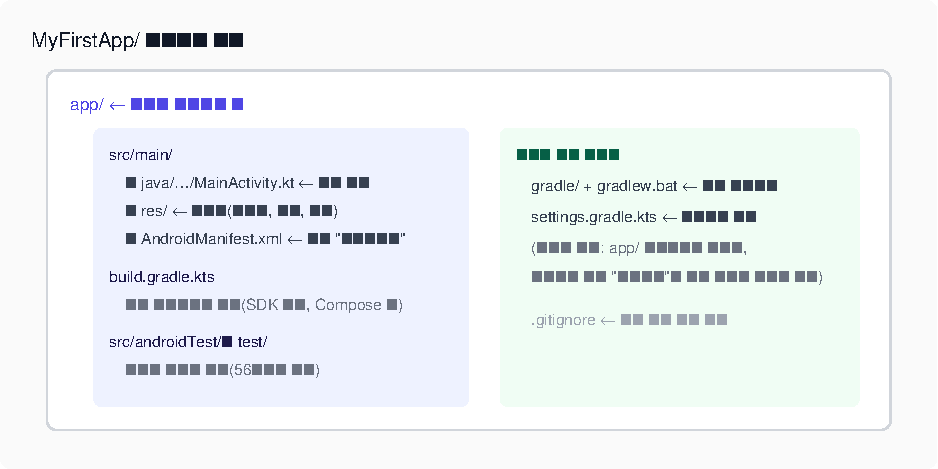
\includegraphics[width=0.92\linewidth]{figures/fig-di-si-shi-jiu-zhang-1}
\\[2pt]\small 그림 2: 초보자가 꼭 알아야 할 프로젝트 구조(주문: app/ 폴더만 다루기)
\end{center}

\begin{itemize}
  \item MainActivity.kt: 앱의 '대문'이에요. 사용자가 아이콘을 누르면 가장 먼저 깨어나는 게 이 파일이죠. 지금 템플릿에서는 "Hello Android!"를 표시하는 일을 맡고 있어요.
  \item AndroidManifest.xml: 앱의 '주민등록부'예요——이 앱의 이름이 무엇인지, 아이콘은 무엇인지, 어떤 화면이 있는지, 어떤 권한(카메라, 위치 등)을 쓰는지 선언해요.
  \item res/ 폴더: 리소스 창고로, 이미지, 아이콘, 문자열, 색을 보관해요. 글자를 코드에 박아 넣지 않고 리소스 파일에 두는 건 안드로이드 개발의 좋은 습관이에요(언어 교체, 테마 교체가 모두 편해요).
  \item build.gradle.kts: 빌드 레시피예요——최소 지원 버전과 어떤 라이브러리(예: Compose)에 의존하는지 선언해요.
\end{itemize}

\booksection{맛보기 실습: “Hello”를 여러분의 이름으로 바꾸기}

MainActivity.kt를 열면 Compose 템플릿이 만들어 준 코드가 보여요. Text(“Hello Android!”) 줄을 찾아 따옴표 안의 글자를 여러분의 이름으로 바꾸세요. 예컨대 Text(“안녕, 철수! 이건 내 첫 앱이야”)처럼요. 그다음 Ctrl+R(Mac은 Cmd+R)을 눌러 다시 실행하세요. 몇 초 뒤 에뮬레이터에 여러분의 이름이 나타나요.

\begin{lstlisting}[language=Kotlin]
setContent {
    MyFirstAppTheme {
        Surface(modifier = Modifier.fillMaxSize()) {
            // v 이곳을 자신의 문자로 바꾸기
            Text("안녕, 김철수! 이게 내 첫 앱이에요")
        }
    }
}
\end{lstlisting}

축하해요, “코드 수정 컴파일 설치 실행”의 온전한 한 바퀴를 완주했어요. 이 반복이야말로 앞으로 매일의 개발 일상이에요. 잘 풀렸으니 이왕 하는 김에 다른 것도 바꿔 보세요: 글자 크기를 키우거나 색을 바꿔 보는 거예요——다음 장에서 이런 '마법'이 어디서 오는지 배우게 돼요.

\booksection{자주 나오는 오류 응급처치: 초보자 첫 2주의 '응급실}

환경 구축과 첫 빌드 단계에서는 아래 세 가지 오류를 만날 가능성이 커요. 놀라지 마세요. 모두 해독제가 있어요:

\begin{center}
\begin{tabularx}{\linewidth}{|X|X|X|}
\hline
\textbf{오류 증상} & \textbf{흔한 원인} & \textbf{해독제} \tabularnewline
\hline
Gradle sync failed / 의존성 내려받기가 느림 & 저장소(리포지터리)에 네트워크 접근이 원활하지 않음 & Gradle에 중국 내 미러 저장소를 설정하세요(알리바바 클라우드/텐센트 클라우드의 maven 미러). 'gradle 중국 미러'로 검색해서 그대로 따라 고치세요 \tabularnewline
SDK 구성 요소 누락 & 설치할 때 SDK 내려받기를 건너뜀 & Settings SDK Manager에서 빠진 플랫폼과 도구를 추가 설치 \tabularnewline
에뮬레이터 시작 실패 / 검은 화면 & 가상화 미사용, 이미지 손상 & BIOS에서 VT-x/AMD-V 켜기; 에뮬레이터를 지우고 다시 만들기; 또는 그냥 실기기 디버깅 사용 \tabularnewline
\hline
\end{tabularx}
\end{center}

\begin{center}\small\color{gray}초보자 환경 오류 응급처치표\end{center}

\begin{tcbinfo}{작은 팁: 오류 검색의 방법론}
오류 메시지의 첫 줄이 가장 가치 있어요——그대로 복사해서 검색 엔진에 넣고 “android studio”라는 키워드를 붙이세요. '환경 설치가 안 돼요 어떡하죠' 같은 두루뭉술한 질문이 아니라 “Gradle sync failed: Could not resolve com.android.tools.build” 같은 구체적인 오류를 검색하는 거예요. 정확한 문제여야 정확한 답이 나와요.

\end{tcbinfo}

\begin{tcbpractice}{따라 해 봐요: '개발 의식감' 체크리스트 완성하기}
(1) Android Studio를 설치하고 에뮬레이터를 돌려 보기; (2) 실기기로 내 앱을 한 번 실행해 보고 스크린샷으로 남기기; (3) Hello 글자를 내 이름으로 바꾸기; (4) 프로젝트를 압축해서 백업해 두기. 이 네 가지를 마치면 SNS에서 이렇게 선언할 수 있어요: 나도 이제 안드로이드 개발자다(스크린샷이 증거).

\end{tcbpractice}

\begin{tcbsummary}{이번 장 정리}
\begin{itemize}
  \item Android Studio = 공식 무료 IDE. 메모리 16GB + 디스크 20GB + 가상화 켜기를 권해요
  \item 새 프로젝트 3요소: 이름, 패키지 이름(전 세계 유일, com.example로 출시 금지), 최소 SDK(API 26부터)
  \item 두 가지 실행 방법: 에뮬레이터(컴퓨터 속 가상 휴대전화)와 실기기(USB 디버깅 켜기, 다 쓰면 끄기)
  \item 프로젝트 주문: app/ 폴더만 다루기——MainActivity.kt는 대문, Manifest는 주민등록부, res/는 리소스 창고
  \item 개발 일상 = 코드 수정 Run 결과 확인의 반복
\end{itemize}

\end{tcbsummary}
